\documentclass[11pt,a4paper]{article}
\usepackage[T1]{fontenc}
\usepackage[utf8]{inputenc}
\usepackage{lmodern}
\usepackage[a4paper,margin=2.4cm]{geometry}
\usepackage{microtype}
\usepackage{setspace}
\usepackage{amsmath}
\usepackage{graphicx}
\usepackage{booktabs,tabularx}
\usepackage[table]{xcolor}
\usepackage{caption}
\usepackage{float}
\usepackage{enumitem}
\usepackage{tikz}
\usetikzlibrary{arrows.meta,positioning}
\usepackage{titlesec}
\usepackage{fancyhdr}
\usepackage{lastpage}
\usepackage[hidelinks]{hyperref}

\graphicspath{{figs/}}
\setstretch{1.15}
\setlength{\parindent}{0pt}
\setlength{\parskip}{0.55em}
\captionsetup{font=small,labelfont=bf,labelsep=period}
\setlist{itemsep=0.15em,topsep=0.3em}
\titleformat{\section}{\normalfont\large\bfseries}{\thesection}{0.8em}{}
\titleformat{\subsection}{\normalfont\normalsize\bfseries}{\thesubsection}{0.8em}{}
\titlespacing*{\section}{0pt}{1.3em}{0.5em}
\titlespacing*{\subsection}{0pt}{0.9em}{0.3em}
\definecolor{boxfill}{HTML}{EEF4F6}
\definecolor{edge}{HTML}{1F6F8B}

\pagestyle{fancy}
\fancyhf{}
\fancyhead[L]{\small\itshape Dahal --- Glacial lake mapping with Sentinel-2}
\fancyhead[R]{\small\itshape Preprint, not peer reviewed}
\fancyfoot[C]{\small \thepage\ of \pageref{LastPage}}
\renewcommand{\headrulewidth}{0.4pt}
\newcommand{\kmsq}{\,km\textsuperscript{2}}

\begin{document}

\begin{center}
{\LARGE\bfseries Mapping glacial lakes in the central Himalaya with Sentinel-2: a spatially held-out comparison of a U-Net and water-index thresholds, with a case study of the Lende--Bhotekoshi floods\par}
\vspace{1.0em}
{\large Subarna Dahal\par}
\vspace{0.3em}
{\small Lalitpur, Nepal\quad$\cdot$\quad \href{mailto:dahalsubarna9@gmail.com}{dahalsubarna9@gmail.com}\par}
{\small Code and results: \url{https://github.com/subarna007/glacial-lake-mapping-sentinel2}\par}
\vspace{0.3em}
{\small Version of 18 November 2026\par}
\end{center}
\vspace{0.4em}
\noindent\rule{\textwidth}{0.4pt}

{\small
\textbf{Abstract}

\textbf{Background.} On 8 July 2025 and again on 26 August 2026 floods came down the Lende river into the Bhotekoshi at Rasuwagadhi, on the Nepal--China border, with almost no warning. Glacial lakes in such remote headwaters can be watched from space for free, but the usual way of mapping them from optical images, a threshold on a water index, is known to struggle with shadows, ice and turbid water.

\textbf{Methods.} I trained a U-Net with a ResNet-34 encoder on post-monsoon Sentinel-2 median composites of the central Himalaya (84.0--88.5\,E), using the hand-checked Hi-MAG 2017 glacial lake inventory as labels. Training, validation and test tiles came from separate longitude strips, so the test lakes lie in mountains the model never saw. The U-Net was compared with NDWI and MNDWI thresholds tuned on the training and validation tiles. The model was then applied, without retraining, to the Lende and upper Bhotekoshi catchments for every autumn from 2017 to 2025, and to every clear single scene around the two floods.

\textbf{Results.} On 160 test tiles (1,049\kmsq) the U-Net reached a pixel IoU of 0.669 (95\% bootstrap interval 0.582--0.737) against 0.490 (0.414--0.570) for NDWI and 0.039 for MNDWI, and found 70.6\% of the 170 test lakes against 45.9\% for NDWI. The gain was largest for lakes of 0.02--0.1\kmsq{} (80.5\% against 50.6\%). The U-Net also produced more water bodies with no matching label (11.5 per 100\kmsq{} against 0.3). In the Lende area, total lake area stayed between 18.5 and 21.0\kmsq{} from 2017 to 2024 and four of the five largest lakes changed by less than 2\%, while one lake near 28.48\,N, 85.74\,E grew every year, from 0.43 to 0.73\kmsq{} (+69\%). No usable cloud-free scene existed between 12 August and 1 October 2026, a seven-week gap that spans the second flood. The 2025 autumn composite failed a band check and was excluded.

\textbf{Conclusions.} A U-Net trained on an existing inventory transfers to unseen parts of the Himalaya and finds clearly more lakes than an index threshold, mostly medium-sized ones. For flood warning, however, the limiting factor in this valley is not the classifier but monsoon cloud: optical images were simply not available when the 2026 flood happened. Combining the optical model with radar (Sentinel-1) is the obvious next step.

\textbf{Keywords:} glacial lakes; GLOF; Sentinel-2; semantic segmentation; U-Net; NDWI; Himalaya; Nepal; Bhotekoshi\par
}
\noindent\rule{\textwidth}{0.4pt}

\section{Introduction}

Glacial lakes in High Mountain Asia have grown in number and size as glaciers retreat \cite{shugar2020,wang2020}. When the moraine or ice that holds such a lake fails, the outburst flood (GLOF) can travel tens of kilometres downstream within an hour. The Bhotekoshi--Trishuli corridor north of Kathmandu is a clear example. On 8 July 2025 a flood from a supraglacial lake on a glacier in Gyirong county, Tibet, came down the Lende river, destroyed the Friendship Bridge at Rasuwagadhi and damaged roads and infrastructure downstream \cite{icimod2025}. On 26 August 2026 the same valley flooded again; early assessments point to an ice avalanche that dammed the Lende near the border and then broke through \cite{icimod2026}. Both times there was almost no warning in Nepal.

The source areas of such floods are high, remote and often across a border, so they are rarely visited. Satellites are the realistic way to watch them. Sentinel-2 images every point of the Himalaya every five days at 10\,m resolution and is free \cite{drusch2012}. The standard way to map lakes in these images is a threshold on a water index such as NDWI \cite{mcfeeters1996} or MNDWI \cite{xu2006}. Thresholds are simple and transparent, but in mountains they mistake terrain shadow for water and miss lakes that are frozen, covered in debris or full of sediment. Deep segmentation networks such as the U-Net \cite{ronneberger2015} can use the shape and surroundings of a lake as well as its colour, and several studies have applied them to glacial lakes \cite{qayyum2020}. What is less often reported is how such a model does on mountains it has not seen, measured against an index threshold that is tuned fairly, and what it actually shows when pointed at a valley that has just flooded.

This paper asks two questions:
\begin{enumerate}[label=\textbf{Q\arabic*.}]
\item How well does a U-Net trained on an existing hand-checked inventory map glacial lakes in Sentinel-2 composites of parts of the Himalaya held out from training, compared with NDWI and MNDWI thresholds?
\item What does the model show for the Lende and upper Bhotekoshi catchments from 2017 to 2025, and around the floods of 2025 and 2026?
\end{enumerate}

The contributions are modest and practical: a fully reproducible pipeline that uses only free data and free computing, a spatially held-out comparison with confidence intervals, and an honest account of where optical monitoring of this valley breaks down.

\section{Data and study area}

\textbf{Images.} I used Sentinel-2 Level-2A surface reflectance \cite{maink2017} from the Microsoft Planetary Computer \cite{pc2022}: the 10\,m bands B2, B3, B4 and B8 and the 20\,m bands B11 and B12, resampled to 10\,m. All images were projected to UTM zone 45N.

\textbf{Labels.} Hi-MAG is an annual inventory of glacial lakes in High Mountain Asia for 2008--2017, mapped from 30\,m Landsat images and checked by hand \cite{chen2021}. I used the 2017 outlines inside 84.0--88.5\,E, 27.6--29.6\,N, which covers the Nepal Himalaya and the Tibetan side of the border.

\textbf{Monitoring area.} A box of 85.15--85.75\,E, 28.20--28.65\,N covers the Lende and upper Bhotekoshi catchments above Rasuwagadhi (Fig.~\ref{fig:lende}a). It was excluded from training altogether.

\section{Methods}

\begin{figure}[H]
\centering
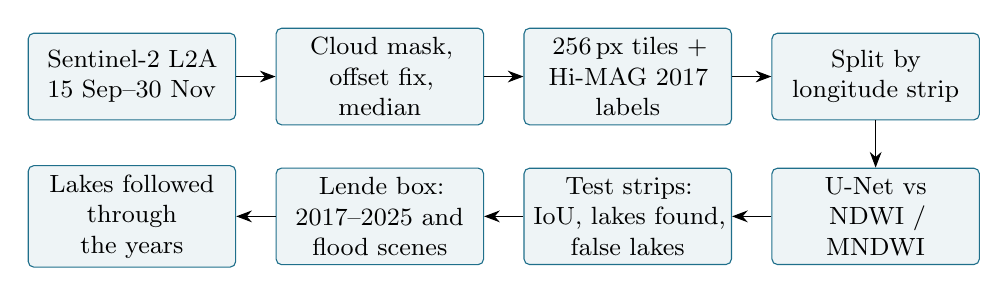
\begin{tikzpicture}[node distance=4mm and 5mm, every node/.style={font=\small},
  box/.style={draw=edge, fill=boxfill, rounded corners=2pt, align=center, minimum height=11mm, text width=24mm}, >={Stealth[length=2mm]}]
\node[box] (a) {Sentinel-2 L2A\\15 Sep--30 Nov};
\node[box, right=of a] (b) {Cloud mask,\\offset fix,\\median};
\node[box, right=of b] (c) {256\,px tiles +\\Hi-MAG 2017\\labels};
\node[box, right=of c] (d) {Split by\\longitude strip};
\node[box, below=of d, yshift=-2mm] (e) {U-Net vs\\NDWI / MNDWI};
\node[box, left=of e] (f) {Test strips:\\IoU, lakes found,\\false lakes};
\node[box, left=of f] (g) {Lende box:\\2017--2025 and\\flood scenes};
\node[box, left=of g] (h) {Lakes followed\\through the years};
\draw[->] (a)--(b); \draw[->] (b)--(c); \draw[->] (c)--(d); \draw[->] (d)--(e);
\draw[->] (e)--(f); \draw[->] (f)--(g); \draw[->] (g)--(h);
\end{tikzpicture}
\caption{Overview of the pipeline.}
\label{fig:pipeline}
\end{figure}

\subsection{Composites}
For each location I took all Sentinel-2 scenes from 15 September to 30 November with less than 40\% cloud in the granule. This post-monsoon window has the least cloud and the least seasonal snow in Nepal. Pixels classed as cloud, cloud shadow, thin cirrus, saturated or missing in the Sen2Cor scene classification layer were masked, and the per-pixel median of the remaining observations was taken. Scenes processed after 25 January 2022 carry a +1000 offset in their digital numbers, which was removed so that all years are on the same scale.

\subsection{Tiles and split}
The study area was divided into tiles of 256$\times$256 pixels (2.56\,km). I sampled up to 900 tiles containing a Hi-MAG lake and half as many lake-free tiles from 2--6 tiles away from a lake, so that the model also sees rivers, shadow, snow and ice that are not lakes. Lake outlines were burnt into each tile as a binary mask.

Neighbouring tiles look alike, so a random split would let the model be tested on near-copies of its training data. Instead tiles were assigned by longitude: test strips at 84.5--85.0\,E and 87.0--87.5\,E, a validation strip at 86.0--86.5\,E, and everything else for training. Tiles within about one tile width of a strip edge were dropped. Tiles with less than 80\% clear pixels were removed, leaving 475 training, 169 validation and 160 test tiles.

\subsection{Models}
\textbf{Index thresholds.} NDWI $=(B3-B8)/(B3+B8)$ \cite{mcfeeters1996} and MNDWI $=(B3-B11)/(B3+B11)$ \cite{xu2006}. For each index the threshold with the highest IoU on all training and validation tiles was chosen from a grid between $-0.4$ and $0.7$ in steps of 0.02. This gives the baselines the same access to labelled data as the network.

\textbf{U-Net.} A U-Net \cite{ronneberger2015} with a ResNet-34 encoder \cite{he2016} pre-trained on ImageNet, with the first layer adapted to six bands (segmentation\_models\_pytorch). Bands were standardised with training-set statistics; missing pixels were set to zero after standardisation and left out of the loss. The loss was binary cross-entropy plus soft Dice. Training ran for 40 epochs with AdamW (learning rate $3\times10^{-4}$, weight decay $10^{-4}$), a cosine schedule, batch size 16, and random 90$^\circ$ rotations and flips. The checkpoint with the best validation IoU (epoch 29) was kept, and the probability threshold (0.65) was chosen on the validation strip.

\subsection{Evaluation}
All scores are on the test strips only. Pixel IoU, F1, precision and recall were computed from true and false positives summed over all observed test pixels; 95\% intervals come from 1,000 bootstrap resamples of tiles \cite{efron1993}. At the lake level, a labelled lake counts as found when at least half of its area is predicted as water, and a predicted water body that touches no labelled lake counts as a false lake. Lakes smaller than 81 pixels (0.0081\kmsq, the Hi-MAG minimum) were not counted at the lake level.

\subsection{Monitoring the Lende area}
The trained model was run over the whole monitoring box (5,942$\times$5,062 pixels) with overlapping 256-pixel windows. Predictions were thresholded and water bodies under 81 pixels removed. To follow lakes through time, each lake is defined as one connected region of the union of all yearly masks; its area in each year is the predicted water inside that region. This keeps one identity for a lake that grows, shrinks or splits. Separately, every single scene from 1 May to 15 August 2025 and from 1 July to 31 October 2026 with at least 60\% clear pixels was processed.

\section{Results}

\subsection{Held-out test strips (Q1)}

\begin{table}[H]
\centering\small
\caption{Results on the held-out test strips (160 tiles, 1,049\kmsq, 170 labelled lakes). Pixel scores are summed over all observed test pixels.}
\label{tab:main}
\begin{tabularx}{\textwidth}{@{}l c c c c c c@{}}
\toprule
Method & Threshold & IoU (95\% CI) & F1 & Precision & Recall & Lakes found \\
\midrule
NDWI & 0.30 & 0.490 (0.414--0.570) & 0.658 & 0.819 & 0.550 & 45.9\% \\
MNDWI & 0.70 & 0.039 (0.015--0.075) & 0.076 & 0.045 & 0.244 & 8.2\% \\
U-Net (ResNet-34) & 0.65 & \textbf{0.669} (0.582--0.737) & \textbf{0.802} & \textbf{0.861} & \textbf{0.750} & \textbf{70.6\%} \\
\bottomrule
\end{tabularx}
\end{table}

The U-Net was better than NDWI on every pixel score (Table~\ref{tab:main}); the bootstrap intervals for IoU overlap only at their ends. NDWI was precise but missed almost half of the lake pixels: lakes that were dark, shadowed or partly frozen fell below its threshold (Fig.~\ref{fig:examples}, rows 1, 4 and 6). MNDWI failed almost completely. Its best threshold on the training tiles sat at the top of the search grid, which means no threshold in the grid could separate water from snow and ice, both of which have high MNDWI values.

\begin{figure}[H]
\centering
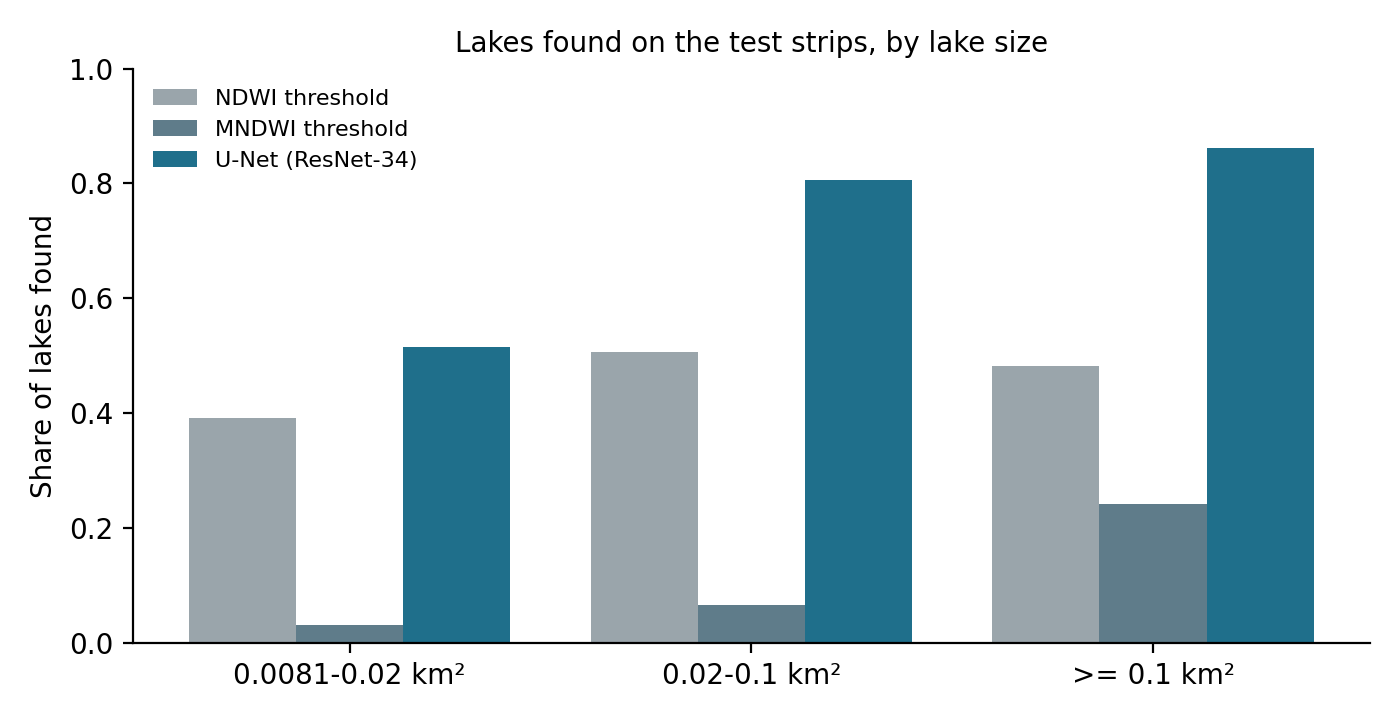
\includegraphics[width=0.82\textwidth]{fig_recall_by_size.png}
\caption{Share of test lakes found, by lake size. Lakes per size class: 64, 77 and 29.}
\label{fig:size}
\end{figure}

Small lakes (0.0081--0.02\kmsq) were the hardest for every method: the U-Net found 51.6\% of them and NDWI 39.1\%. The largest gain was for lakes of 0.02--0.1\kmsq{}, where the U-Net found 80.5\% against 50.6\%. For lakes of at least 0.1\kmsq{} the U-Net found 86.2\% (Fig.~\ref{fig:size}).

The U-Net paid for its higher recall with more false lakes: 11.5 per 100\kmsq{} against 0.3 for NDWI. Some of these are true errors, but Fig.~\ref{fig:examples} shows another cause. Where every scene in the composite was masked, the network sometimes predicted a lake inside the gap (row 3, bottom right). These gaps are often dark lakes that the Sen2Cor classifier labelled as cloud shadow, so the network is partly right for the wrong reason. Pixel scores ignore such gaps, but the lake-level scores in this first run did not; the evaluation code has since been changed to ignore predictions in gaps, and the lake-level numbers should be read with this in mind.

\begin{figure}[!htbp]
\centering
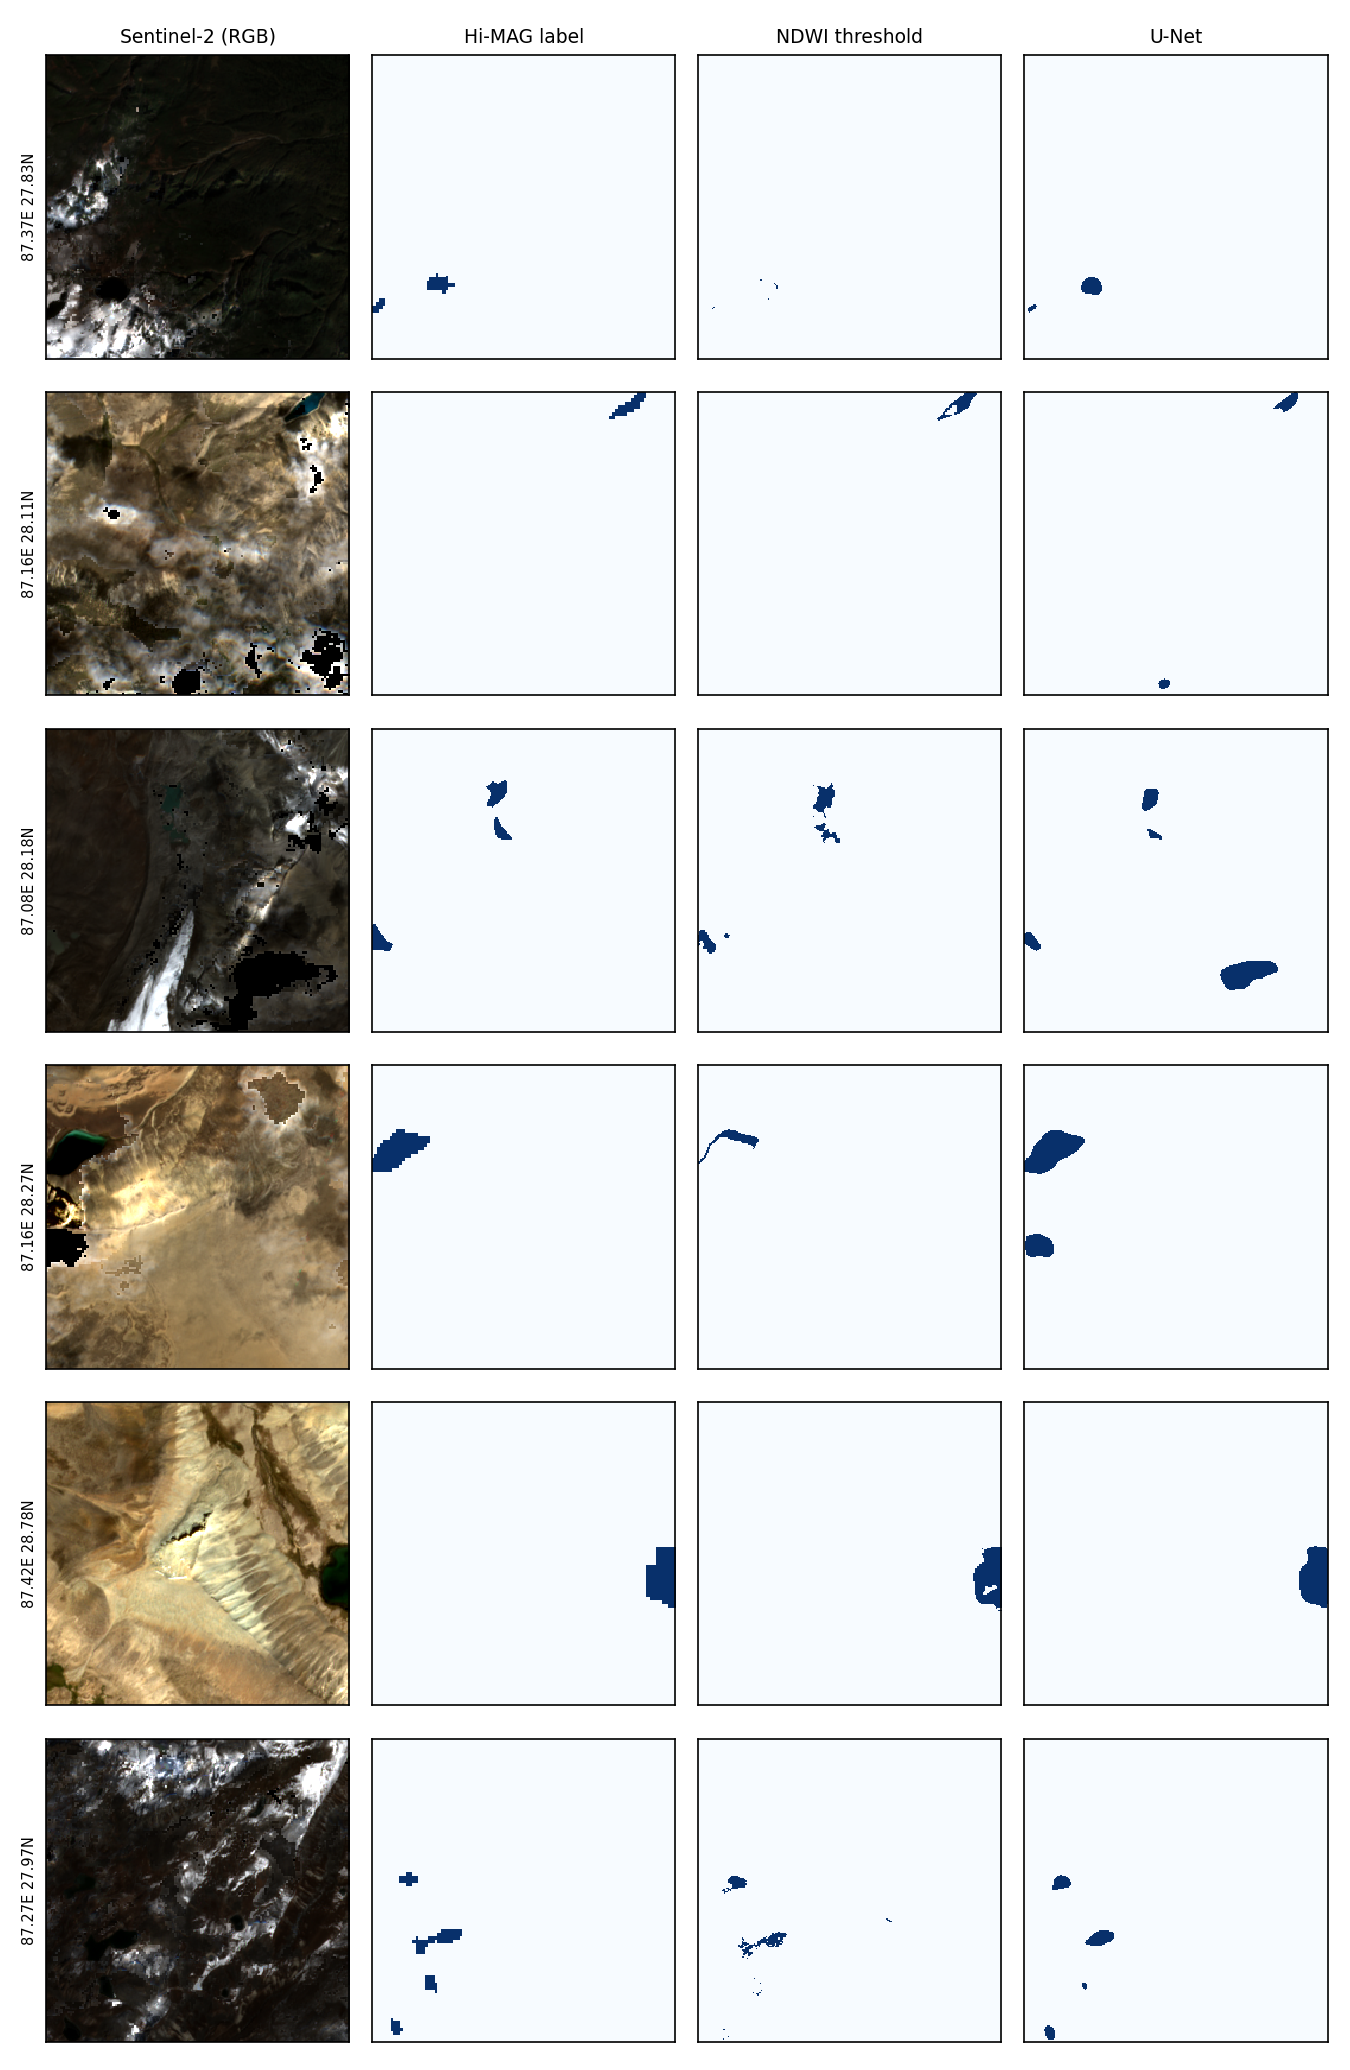
\includegraphics[width=0.58\textwidth]{fig_examples.png}
\caption{Six randomly chosen test tiles with lakes. Black areas in the image are pixels with no clear observation.}
\label{fig:examples}
\end{figure}

\subsection{Lende and upper Bhotekoshi (Q2)}

\begin{figure}[H]
\centering
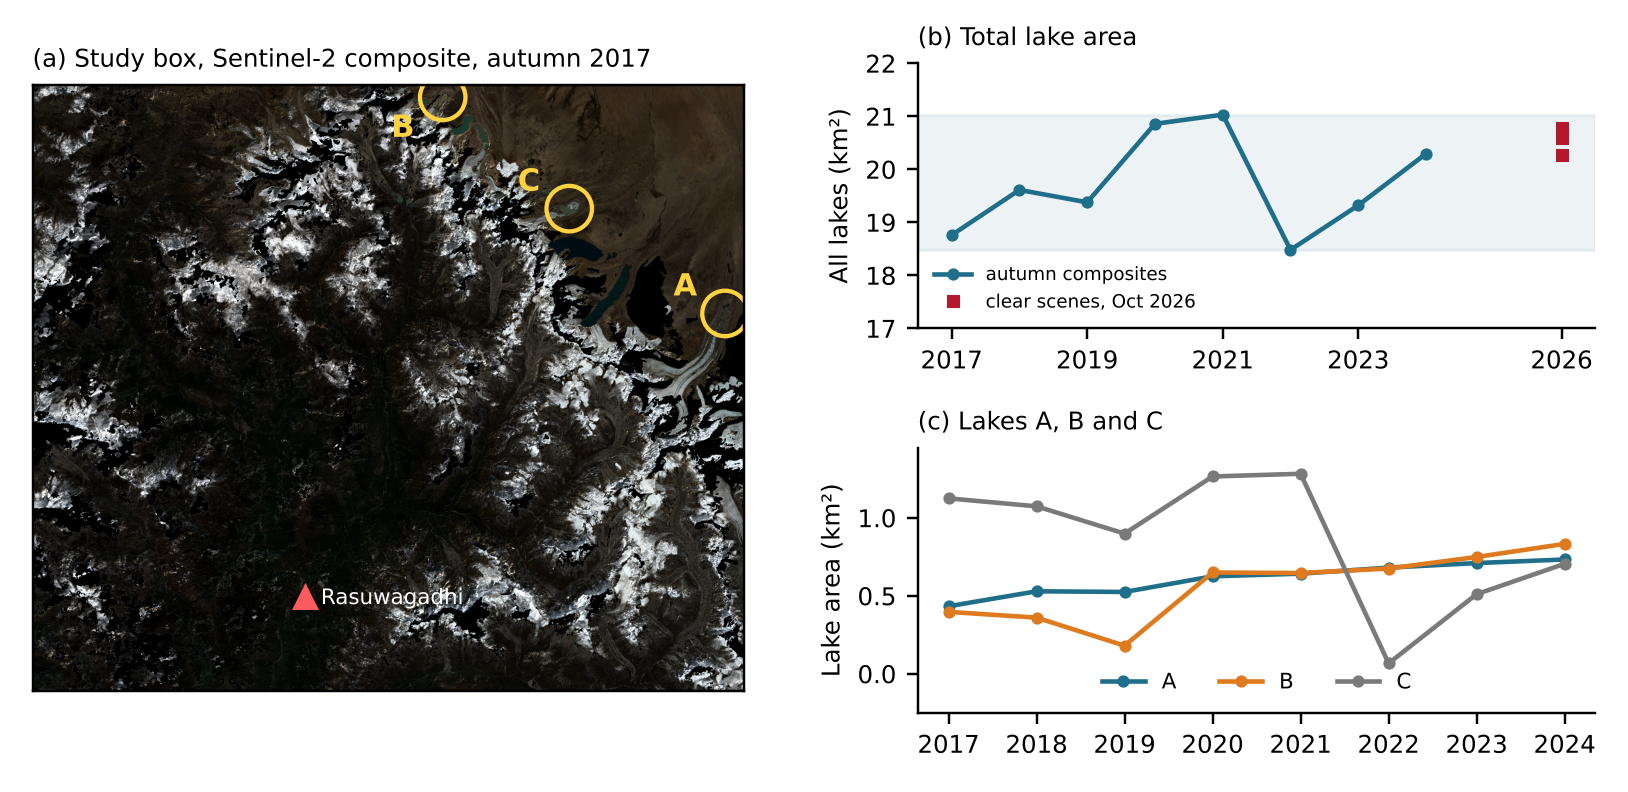
\includegraphics[width=\textwidth]{fig_lende.png}
\caption{(a) Monitoring box with the three lakes discussed in the text. (b) Total mapped lake area per autumn, 2017--2024 (shaded: range), and the three full-coverage clear scenes after the 2026 flood. (c) Area of lakes A, B and C.}
\label{fig:lende}
\end{figure}

\textbf{Year to year.} Between 2017 and 2024 the model mapped 72--91 lakes per autumn with a total area of 18.5--21.0\kmsq{} (mean 19.7, SD 0.9; Fig.~\ref{fig:lende}b). There was no steady trend. Four of the five largest lakes, which together hold about 60\% of the mapped area, changed by less than 2\% between 2017 and 2024, with a year-to-year coefficient of variation of 0.2--1.4\%; the model gives consistent outlines for the same lake from different images. The fifth is lake C, discussed below. Forty-four lakes were found in all eight years and held 92\% of the mapped area; 116 small water bodies appeared in only one or two years and together averaged 0.19\kmsq.

\textbf{Lakes that changed.} Lake A (28.483\,N, 85.735\,E) grew in every year, from 0.43\kmsq{} in 2017 to 0.73\kmsq{} in 2024 (+69\%). Lake B (28.642\,N, 85.490\,E) roughly doubled, from 0.40 to 0.83\kmsq{}, with a jump in 2020. Lake C (28.562\,N, 85.600\,E) is an example of what not to trust: its area dropped to 0.07\kmsq{} in 2022 and recovered, which is far more likely to be ice or snow on the lake in that year's composite than a real change. Lake A lies within about 1.5\,km of the east edge of the box, so part of it may fall outside the mapped area.

\textbf{2025.} The autumn 2025 composite came out with near-zero red and green and very high blue reflectance across the whole box, which is not physically possible. The model mapped only 11.2\kmsq{} of lakes on it. Single scenes from the same year looked normal, so the fault lies in the data read for that composite, not in the landscape. This year was excluded, and the pipeline now rejects composites whose band medians are implausible and masks reflectance above 1.5.

\textbf{Around the floods.} Before the July 2025 flood, the scenes that passed the clear-pixel filter covered only part of the box: the satellite's swath edge runs through it, and in May and June many lakes were still frozen or snow covered. The mapped lake area of these scenes ranged from 0.3 to 19.3\kmsq{}, which reflects coverage and ice, not lakes filling and draining, so they cannot answer whether the source lake was visible beforehand. For 2026 the result is clearer. The last usable scene before the flood was on 12 August, and the next one on 1 October: for seven weeks, including the day of the flood, there was no clear optical view of the valley. After the flood, the three scenes covering the whole box (1, 21 and 26 October) gave 20.3, 20.6 and 20.8\kmsq{}, inside the 2017--2024 range. This is consistent with the 2026 flood not having drained one of the large lakes, but a few hundredths of a square kilometre could easily be lost in this comparison.

\section{Discussion}

\textbf{What the U-Net adds.} Trained on one inventory and tested on separate mountains, the network found about one and a half times as many lakes as the best index threshold. The gain was concentrated in lakes of 0.02--0.1\kmsq{}, which are numerous and which thresholds miss when they are dark or partly frozen. This matters because small and medium lakes are the ones least likely to be in older inventories.

\textbf{Why MNDWI failed.} MNDWI is usually considered more robust than NDWI over built-up land, but in glaciated terrain snow and ice also reflect strongly in green and weakly in short-wave infrared, so they look like water. In tiles dominated by snow no single threshold works. This is a known problem and a reminder that indices must be checked in the setting where they will be used.

\textbf{Limits of the labels.} Hi-MAG outlines come from 30\,m Landsat pixels and from one scene per lake between July and November 2017, while my images are a 10\,m median of September--November. Blocky label edges and real changes within the season both count as errors, so an IoU of 0.67 is a lower bound on how well the outlines match reality.

\textbf{Cloud masks remove dark lakes.} A good share of the gaps in the composites sit on lakes. Sen2Cor sometimes labels dark water as cloud shadow, and after masking every scene the lake is simply missing. A mask designed for mountains, or one that does not drop pixels classed as shadow when the same pixel is water in other scenes, would recover these lakes for every method.

\textbf{What this means for warnings.} The main lesson from the Lende case is not about the classifier. The 2026 flood happened in the middle of a seven-week period with no clear optical image, and the 2025 source was a short-lived summer lake that an autumn composite cannot show. Optical satellites are blind in the monsoon, which is when lakes are fullest and floods most likely.

\section{What can be explored next}
\begin{itemize}
\item \textbf{Radar.} Sentinel-1 radar sees through cloud \cite{torres2012}. Training the same model on Sentinel-1, or on both sensors together, would give images during the monsoon.
\item \textbf{The 2025 source lake.} Locating the Purepu supraglacial lake and following it scene by scene through June and July 2025 would show whether it was visible before it drained, and for how long.
\item \textbf{Terrain inputs.} Adding elevation and slope from a digital elevation model would help separate lakes from shadow and from rivers on steep valley floors.
\item \textbf{Several dates at once.} A model that looks at a stack of scenes, rather than one median, could use the fact that shadows move and lakes do not.
\item \textbf{Newer labels.} Training on more recent or 10\,m inventories would remove much of the label mismatch.
\item \textbf{Wider testing.} Other basins of Nepal and the Tibetan plateau, and a second random seed and encoder, would show how stable the results are.
\end{itemize}

\section{Limitations}
One training run with one seed; one label year; test strips in the central Himalaya only; lake-level scores from the first run counted predictions inside data gaps (fixed in the code, not yet re-run); the 2025 autumn composite was unusable; and nothing here has been checked on the ground.

\section{Conclusion}
A U-Net trained on an existing hand-checked inventory maps glacial lakes in unseen parts of the Himalaya clearly better than water-index thresholds, especially medium-sized lakes, at the cost of more false detections. Applied to the Lende and upper Bhotekoshi catchments, it gives stable outlines for the large lakes over eight years and points to two lakes that grew steadily. It could not have warned of either flood, because no clear optical image existed at the time. Monitoring that works in the monsoon will need radar.

\section*{Data and code availability}
Sentinel-2 data are free from the Copernicus programme via the Microsoft Planetary Computer. Hi-MAG is available from Zenodo (\url{https://zenodo.org/records/4275164}). All code, metrics, tables and figures are at \url{https://github.com/subarna007/glacial-lake-mapping-sentinel2}.

\begin{thebibliography}{99}\small
\bibitem{shugar2020} Shugar DH, Burr A, Haritashya UK, Kargel JS, Watson CS, Kennedy MC, et al. Rapid worldwide growth of glacial lakes since 1990. Nature Climate Change. 2020;10:939--945.
\bibitem{wang2020} Wang X, Guo X, Yang C, Liu Q, Wei J, Zhang Y, et al. Glacial lake inventory of high-mountain Asia in 1990 and 2018 derived from Landsat images. Earth System Science Data. 2020;12:2169--2182.
\bibitem{icimod2025} ICIMOD. Situation updates on the Rasuwa flood of 8 July 2025. International Centre for Integrated Mountain Development; 2025. \url{https://www.icimod.org}
\bibitem{icimod2026} ICIMOD. Situation updates on the Bhotekoshi flood of 26 August 2026. International Centre for Integrated Mountain Development; 2026. \url{https://www.icimod.org}
\bibitem{drusch2012} Drusch M, Del Bello U, Carlier S, Colin O, Fernandez V, Gascon F, et al. Sentinel-2: ESA's optical high-resolution mission for GMES operational services. Remote Sensing of Environment. 2012;120:25--36.
\bibitem{mcfeeters1996} McFeeters SK. The use of the Normalized Difference Water Index (NDWI) in the delineation of open water features. International Journal of Remote Sensing. 1996;17(7):1425--1432.
\bibitem{xu2006} Xu H. Modification of normalised difference water index (NDWI) to enhance open water features in remotely sensed imagery. International Journal of Remote Sensing. 2006;27(14):3025--3033.
\bibitem{ronneberger2015} Ronneberger O, Fischer P, Brox T. U-Net: convolutional networks for biomedical image segmentation. In: MICCAI 2015. Springer; 2015. p. 234--241.
\bibitem{qayyum2020} Qayyum N, Ghuffar S, Ahmad HM, Yousaf A, Shahid I. Glacial lakes mapping using multi satellite PlanetScope imagery and deep learning. ISPRS International Journal of Geo-Information. 2020;9(10):560.
\bibitem{maink2017} Main-Knorn M, Pflug B, Louis J, Debaecker V, M\"uller-Wilm U, Gascon F. Sen2Cor for Sentinel-2. In: Proc. SPIE 10427, Image and Signal Processing for Remote Sensing XXIII; 2017.
\bibitem{pc2022} Microsoft Open Source, McFarland M, Emanuele R, Morris D, Augspurger T. microsoft/PlanetaryComputer. Zenodo; 2022. \url{https://planetarycomputer.microsoft.com}
\bibitem{chen2021} Chen F, Zhang M, Guo H, Allen S, Kargel JS, Haritashya UK, et al. Annual 30\,m dataset for glacial lakes in High Mountain Asia from 2008 to 2017. Earth System Science Data. 2021;13:741--766. doi: 10.5194/essd-13-741-2021
\bibitem{he2016} He K, Zhang X, Ren S, Sun J. Deep residual learning for image recognition. In: CVPR 2016. p. 770--778.
\bibitem{efron1993} Efron B, Tibshirani RJ. An introduction to the bootstrap. Chapman and Hall; 1993.
\bibitem{torres2012} Torres R, Snoeij P, Geudtner D, Bibby D, Davidson M, Attema E, et al. GMES Sentinel-1 mission. Remote Sensing of Environment. 2012;120:9--24.
\end{thebibliography}

\end{document}
